% This is samplepaper.tex, a sample chapter demonstrating the
% LLNCS macro package for Springer Computer Science proceedings;
% Version 2.20 of 2017/10/04
%
\documentclass[runningheads]{llncs}
%
\usepackage{graphicx}
\usepackage{url}
\usepackage[scale=0.69]{geometry}
% Used for displaying a sample figure. If possible, figure files should
% be included in EPS format.
%
% If you use the hyperref package, please uncomment the following line
% to display URLs in blue roman font according to Springer's eBook style:
% \renewcommand\UrlFont{\color{blue}\rmfamily}

\newcommand{\Jupyter}{\textbf{Jupyter}}

\begin{document}
%
\title{Proposition d'atelier : introduction au merveilleux écosystème des notebooks \Jupyter{} pour l'enseignement et des travaux pratiques en informatique}
% \thanks{Supported by ENS Rennes and CentraleSup{\'e}lec.}}
%
\titlerunning{Introduction aux notebooks \Jupyter}
% If the paper title is too long for the running head, you can set
% an abbreviated paper title here
%
% \author{Lilian Besson\inst{1}\orcidID{0000-0003-2767-2563}}
% %
% \authorrunning{Lilian Besson}
% % First names are abbreviated in the running head.
% % If there are more than two authors, 'et al.' is used.
% %
% \institute{{\'E}cole Normale Sup{\'e}rieure de Rennes, Bruz, France\\
% \email{lilian.besson{@}ens-rennes.fr}\\
% \url{www.ens-rennes.fr/}}
%
\maketitle              % typeset the header of the contribution
%
\begin{abstract}
    % https://www.didapro.org/8/contributions-dates/

    Je propose un tutoriel qui présentera les notebooks \Jupyter{} et donnera un bon aperçu du grand écosystème \Jupyter{}.
    Les ressources de ce tutoriel sont présentes en lignes sur \texttt{http://frama.link/Atelier-Jupyter-Didapro8}

    Je vais expliquer et montrer comment on peut facilement (et gratuitement) utiliser les portables \Jupyter{} avec le langage de programmation Python, ainsi que d'autres langages.
    % Notebooks can be used for lecture material, to obtain one document that contains text, maths, figures, code snippets and the outputs of their execution.
    Les notebooks peuvent être utilisés pour du matériel de cours, pour obtenir un document qui contient du texte, des maths, des figures, des extraits de code et les résultats de leurs exécutions.
    % \Jupyter{} Notebooks are also an excellent tool to use for practical sessions in studying computer science, but also any other science with numerical computations or data analysis (mathematics, physics and chemistry, engineering etc), as a template or a skeleton can be given to the students, and collected and rated after the practical session.
    Les notebooks \Jupyter{} sont également un excellent outil pour les travaux pratiques d'informatique, mais aussi pour toute autre science avec des calculs numériques ou l'analyse de données (mathématiques, physique et chimie, ingénierie, etc), et comme modèle ou squelette pouvant être remis aux étudiants, et collectés et évalués après la session pratique.

    J'illustre ces outils et présente comment écrire des cahiers propres et jolis, comment les convertir en HTML, code source ou PDF, en détaillant mon utilisation quotidienne de l'écosystème \Jupyter{} en tant que professeur d'informatique dans le supérieur.
    % à l'ENS de Rennes.
    J'utilise des notebooks \Jupyter, pour des enseignements du niveau L3 à M2, depuis trois ans, et je veux partager cette expertise avec d'autres enseignants en informatique.
    Mes documents sont open-source et publiés en ligne, et sont utilisés pour un cours sur les algorithmes (L3), et pour la formation à l'option informatique à l'examen national de l'agrégation de mathématiques.

    % The abstract should briefly summarize the contents of the paper in 150--250 words.

% \keywords{Jupyter \and Notebook \and Python \and Open-source tool \and Teaching programming \and Data science.}
    \keywords{Jupyter \and Notebook \and Python \and Outil open-source \and Enseignement de la programmation \and Enseignement de l'informatique \and Science des données.}
\end{abstract}
%
%
%

% -------------------------
% \section{Outline of the tutorial content}

% In 30 minutes, and as many times as possible on the Wednesday 7th of February, the author proposes to present the following points.

\section{Aperçu du contenu du tutoriel}

En une heure, et une ou deux sessions le mercredi 5 février, l'auteur propose de présenter les points suivants.


% \subsection*{Presentation of \Jupyter}
\subsection*{Présentation de \Jupyter}


\begin{itemize}
    \item Qu'est-ce qu'un notebook \Jupyter{} : un environnement de développement intégré (IDE) ``WYSIWYG'' (What-you-see-is-what-you-get) pour (presque) tous les langages de programmation. Par exemple, il peut être utilisé pour des langages dynamiques interprétés, tels que Python \cite{python}, OCaml\footnote{Avec \url{github.com/akabe/ocaml-jupyter}, et d'autres ``noyaux'' pour d'autres langages.}, Julia ou Bash, mais aussi pour des langages compilés, tels que C/C++ etc.

    \item Qu'est-ce que l'écosystème \Jupyter{} : il a commencé sous le nom \texttt{ipython} \cite{ipython} il y a environ 10 ans, conçu pour être utilisé uniquement pour le langage de programmation Python, et de nos jours il a évolué en un écosystème open-source mature.
    Il est utilisé par des centaines de milliers de scientifiques du monde entier, et parmi ses récentes utilisations réussies, on peut noter la toute première image d'un trou noir par Katie Bouman et ses collaborateurs\footnote{Voir par exemple \url{www.nationalgeographic.com/science/2019/04/first-picture-black-hole-revealed}\\\url{-m87-event-horizon-telescope-astrophysics/} et \url{www.bbc.com/news/science-environment-47891902}.}, ou par des lauréats de prix Nobel, comme Paul Romer\footnote{Voir \url{paulromer.net/jupyter-mathematica-and-the-future-of-the-research-paper/}}.
    Les notebooks \Jupyter{} sont une alternative gratuite et open-source à l'EDI propriétaire inclus dans les logiciels MATLAB, Wolfram's Mathematica et MapleSoft's Maple.

    \item Quels problèmes résolvent les notebooks \Jupyter{} ? Pourquoi c'est un outil puissant, à la fois facile à apprendre et à utiliser pour les débutants et puissant pour les utilisateurs experts.
\end{itemize}



\subsection*{Comment installer \Jupyter{}}

En suivant le tutoriel en ligne depuis \url{jupyter.org/install.html}, il est facile d'installer tout l'écosystème \Jupyter{} sur tout ordinateur avec Python et \texttt{pip} ou \texttt{conda} installés.


\subsection*{Comment utiliser \Jupyter{} pour écrire des documents simples}

Le tutoriel montrera l'interface utilisateur graphique des notebooks \Jupyter{}.
Je montrerai également les pages du tutoriel et de la documentation officiels en ligne, qui vous permettront d'apprendre par vous-même si besoin.


\subsection*{Présentant ma propre utilisation de Jupyter{} notebooks}

Je vais montrer comment j'utilise des cahiers Jupyter au quotidien pour mes activités d'enseignement, durant les trois dernières années.
Je présenterai principalement des exemples de ressources produites à partir d'un notebook \Jupyter{}, et comment convertir des notebooks en HTML.

\begin{itemize}
    \item
    J'ai utilisé des notebooks \Jupyter{} pour écrire les sujets et les solutions des sessions pratiques utilisées pour entraîner nos étudiants à l'examen oral de modélisation de l'agrégation.
    Voir \url{nbviewer.jupyter.org/github/Naereen/notebooks/tree/master/agreg/TP_Programmation_2017-18/},
    avec le langage \textbf{OCaml}, pour des étudiants de M2.

    \begin{figure}[!h]
        \centering
        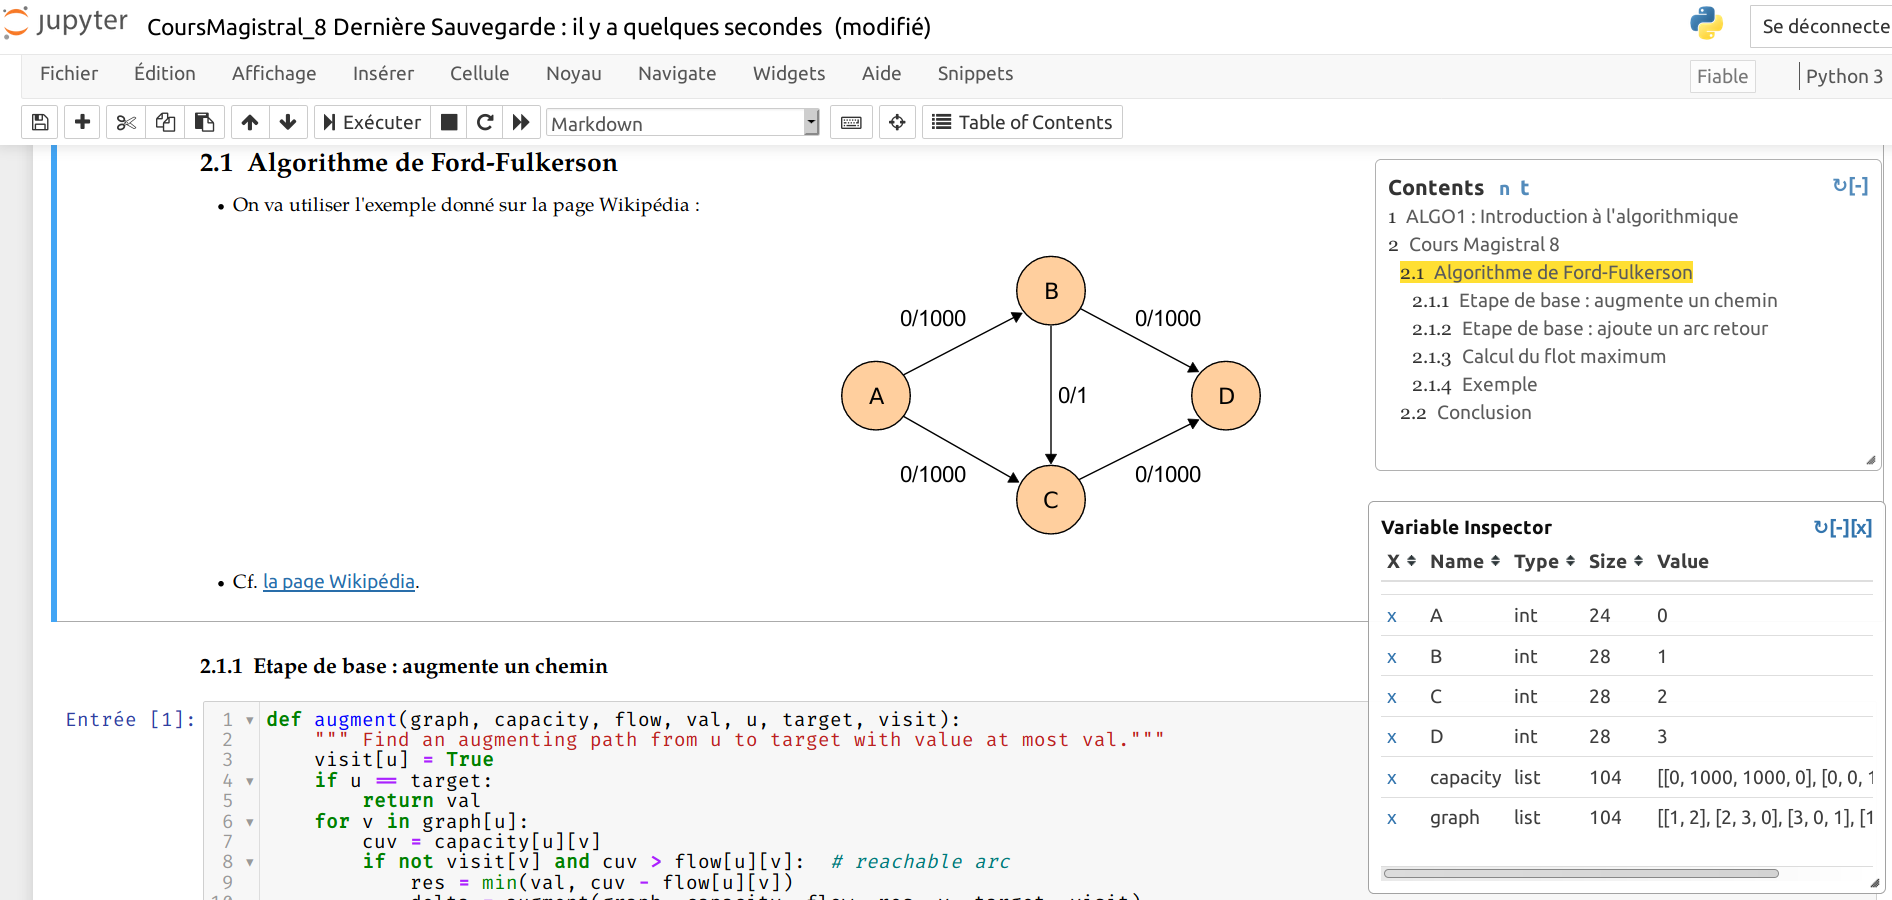
\includegraphics[width=10cm]{apercu_ENS_agreg_4.png}
        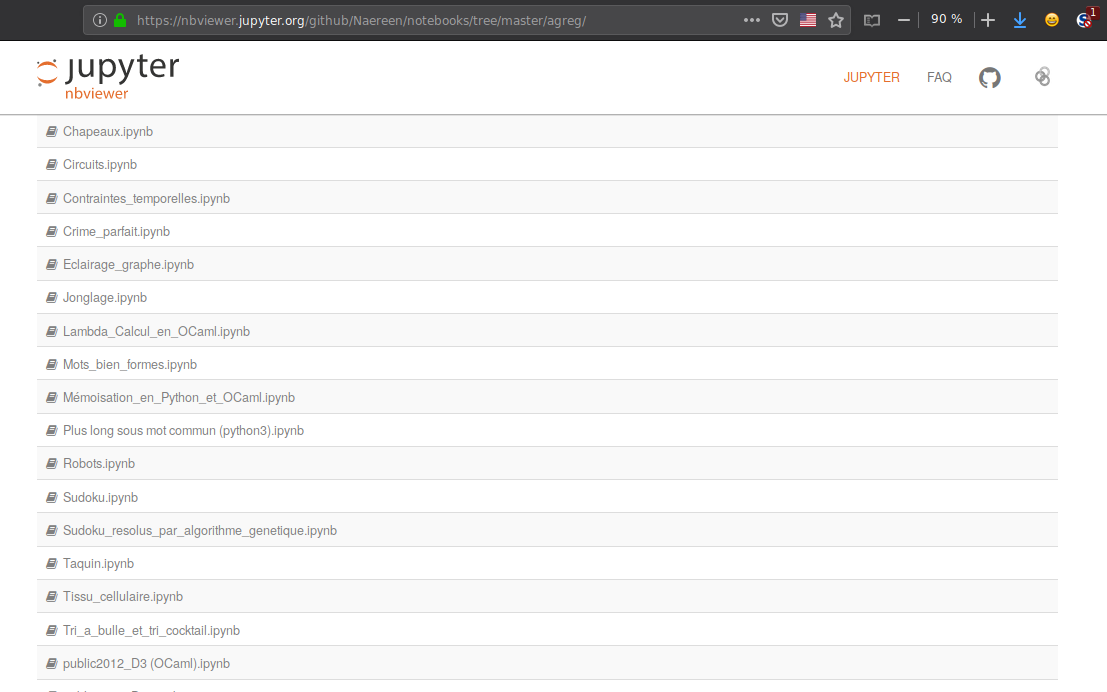
\includegraphics[width=6cm]{apercu_ENS_agreg_1.png}
        % 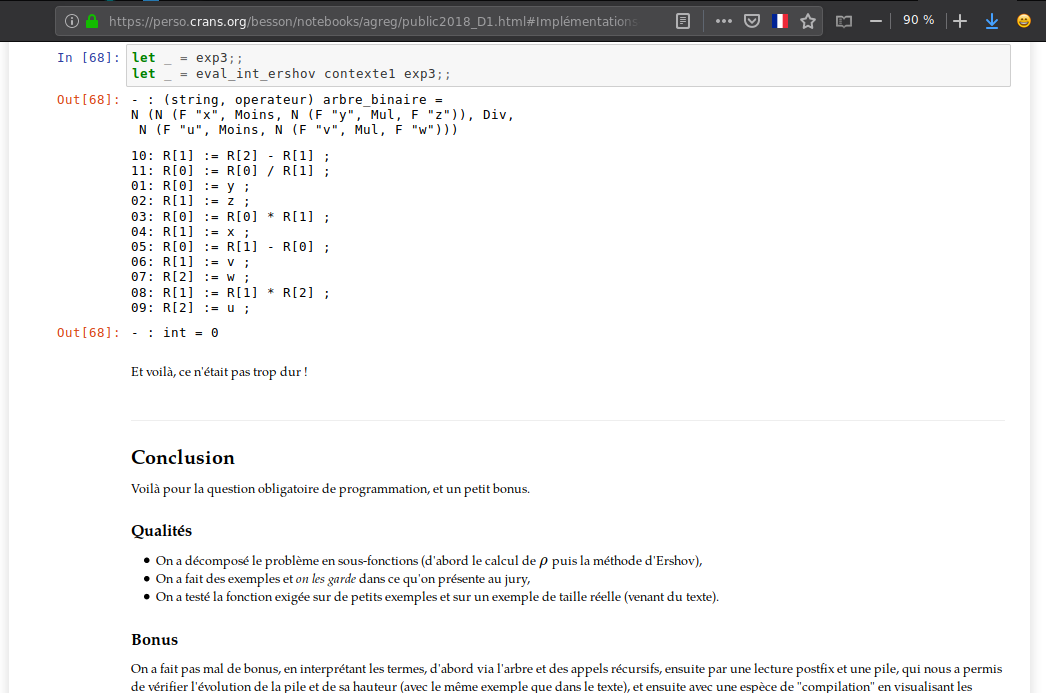
\includegraphics[width=6cm]{apercu_ENS_agreg_2.png}
        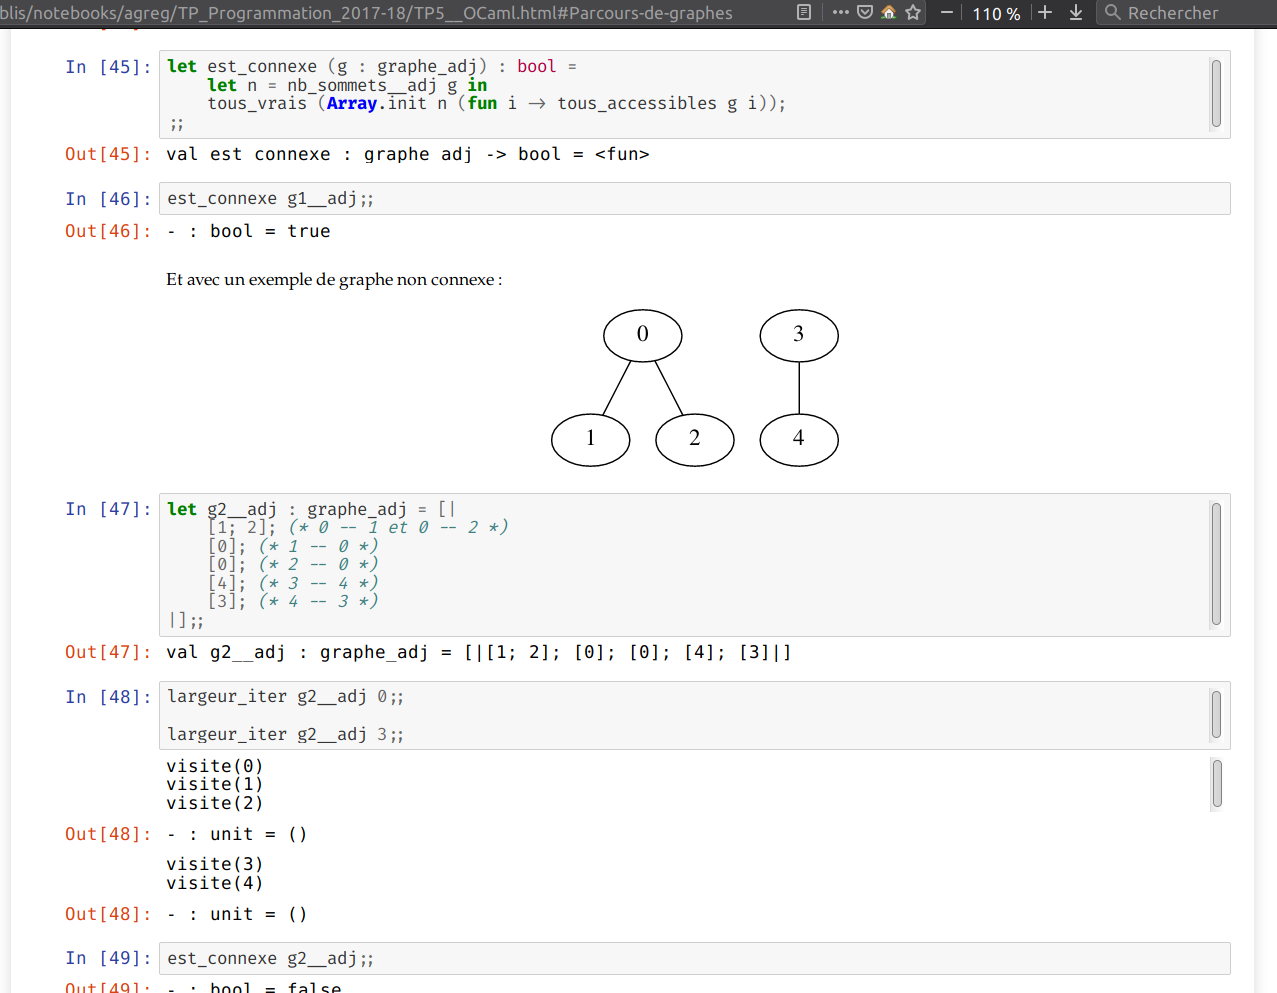
\includegraphics[width=6cm]{apercu_ENS_agreg_3.png}
        \caption{Exemples d'utilisation de notebooks \Jupyter.}
        \label{}
    \end{figure}


    \item
    J'ai écrit des implémentations propres et détaillées de structures de données et d'algorithmes, partant de rien, pour un cours d'algorithmique à l'automne 2019, avec des notebooks \Jupyter.
    Voir \url{github.com/Naereen/ALGO1-Info1-2019/},
    avec le langage \textbf{Python}, pour des étudiants de L3.

    \item
    J'ai écrit les solutions pour les sessions pratiques données en tant qu'entraînement pour l'examen oral ``Mathématiques avec Python'' du concours CentraleSupélec (CPGE), avec des notebooks \Jupyter, afin de les partager facilement avec les étudiants, de les exposer et de travailler dessus pendant les sessions pratiques.
    Voir \url{perso.crans.org/besson/notebooks/Oraux_CentraleSupelec_PSI__Juin_2019.html},
    avec \textbf{Python} et des maths,
    pour les étudiants d'une classe du PSI (CPGE) en juin 2017, 2018 et 2019.

    \item
    Avec un collègue, nous avons donné un tutoriel d'une heure présentant le langage de programmation \textbf{Julia}, lors d'un séminaire annuel d'un grand laboratoire de recherche en juin 2018 à Vannes, pour environ 50 personnes.
    Nous avons utilisé deux notebooks \Jupyter{} pendant le séminaire \url{github.com/pierre-haessig/julia-presentation-ietr2018/},
    et ces diapositives \url{hal.archives-ouvertes.fr/cel-01830248/}.

\end{itemize}


% \subsection*{Pointers on how to become a \Jupyter{} expert}
\subsection*{Des conseils pour devenir un expert en \Jupyter}

L'atelier contiendra également des liens pour maîtriser l'écosystème \Jupyter{} et les utiliser pour votre propre projet.

\begin{itemize}
    \item Comment utiliser un dépôt GitHub/Bitbucket/GitLab pour héberger des notebooks \Jupyter{}, et les afficher en ligne en utilisant le site \url{nbviewer.jupyter.org/}.
    Voir \url{github.com/Naereen/ALGO1-Info1-2019/} et \url{github.com/Naereen/notebooks/}
    \item Utilisez Binder, Google Colab ou d'autres outils gratuits en ligne, pour ajouter un lien afin que tout utilisateur consultant vos notebooks \Jupyter{} puisse démarrer un environnement interactif, directement depuis son navigateur Web, pour interagir avec le notebook sans rien avoir à installer.
    \item Utilisez les extensions \Jupyter{} pour améliorer l'EDI, par exemple pour ajouter automatiquement une table des matières. Voir \url{jupyter-contrib-nbextensions.readthedocs.io/en/latest/}.
    \item Suivre les meilleurs exemples, par exemple le célèbre Peter Norvig publie des notebooks très intéressants sur son projet \url{github.com/norvig/pytudes}, depuis 5 ans.
    \item Partagez vos notebooks en ligne, avec vos étudiants et collègues, et recevez leurs commentaires.
\end{itemize}


% -------------------------
\section{Détails techniques}

Nous énumérons le matériel nécessaire pour le tutoriel, ainsi que d'autres détails techniques.

\subsection*{Matériel}

\begin{itemize}
    \item Chaque participant doit venir avec son propre ordinateur portable.
    \item C'est mieux si l'écosystème \Jupyter{} est déjà installé.
    \item Un grand écran et un projecteur pour l'intervenant.
\end{itemize}


\subsection*{Autres détails}

\begin{itemize}
    \item Il n'y a pas de limite en termes de nombre de personnes pouvant assister à ce tutoriel, sauf la limitation de la salle.
    \item Notez qu'aucune connaissance préalable du langage Python n'est nécessaire pour utiliser les notebooks \Jupyter.
\end{itemize}



% -------------------------
\section{Session pratique}

J'utiliserai, bien sûr, un notebook \Jupyter{} comme matériel affiché pendant le tutoriel (l'exposé lui-même est donc un méta-exemple).
Pour les personnes qui assisteront au séminaire, et pour les personnes curieuses qui le manqueront, je partagerai le notebook de présentation en ligne au préalable.

Le tutoriel contiendra également un ``travail à domicile'' pour les personnes intéressées, comme un notebooks avec des trous à remplir, et des tâches à résoudre.
Je proposerai de relire les notebooks remplis, si quelqu'un veut me l'envoyer, et d'offrir une aide par courriel si nécessaire (même si StackOverflow fait un bien meilleur travail que quiconque).


% ---- Bibliography ----
%
% BibTeX users should specify bibliography style 'splncs04'.
% References will then be sorted and formatted in the correct style.
%
% \bibliographystyle{splncs04}
% \bibliography{mybibliography}
%
\begin{thebibliography}{8}
    \bibitem{jupyter}
    Thomas Kluyver et al.
    \textbf{Jupyter Notebooks - a publishing format for reproducible computational workflows}.
    In F. Loizides and B. Schmidt, editors, Positioning and Power in Academic Publishing: Players, Agents and Agendas, pages 87–90. IOS Press, 2016.

    \bibitem{python}
    Python Software Foundation.
    \textbf{Python Language Reference}, version 3.6, October 2017. \url{www.python.org}.

    \bibitem{ipython}
    Fernando Pérez and Brian E. Granger.
    \textbf{IPython: a System for Interactive Scientific Computing}.
    \emph{Computing in Science and Engineering}, 9(3):21–29, May 2007. ISSN 1521-9615. \url{ipython.org}.
\end{thebibliography}
\end{document}
